% Options for packages loaded elsewhere
\PassOptionsToPackage{unicode}{hyperref}
\PassOptionsToPackage{hyphens}{url}
\PassOptionsToPackage{dvipsnames,svgnames,x11names}{xcolor}
\PassOptionsToPackage{space}{xeCJK}
\documentclass[
  a4paper,12pt]{article}
\usepackage{xcolor}
\usepackage[margin=2.5cm]{geometry}
\usepackage{amsmath,amssymb}
\setcounter{secnumdepth}{5}
\usepackage{iftex}
\ifPDFTeX
  \usepackage[T1]{fontenc}
  \usepackage[utf8]{inputenc}
  \usepackage{textcomp} % provide euro and other symbols
\else % if luatex or xetex
  \usepackage{unicode-math} % this also loads fontspec
  \defaultfontfeatures{Scale=MatchLowercase}
  \defaultfontfeatures[\rmfamily]{Ligatures=TeX,Scale=1}
\fi
\usepackage{lmodern}
\ifPDFTeX\else
  % xetex/luatex font selection
  \ifXeTeX
    \usepackage{xeCJK}
    \setCJKmainfont[]{Songti SC}
  \fi
  \ifLuaTeX
    \usepackage[]{luatexja-fontspec}
    \setmainjfont[]{Songti SC}
  \fi
\fi
% Use upquote if available, for straight quotes in verbatim environments
\IfFileExists{upquote.sty}{\usepackage{upquote}}{}
\IfFileExists{microtype.sty}{% use microtype if available
  \usepackage[]{microtype}
  \UseMicrotypeSet[protrusion]{basicmath} % disable protrusion for tt fonts
}{}
\makeatletter
\@ifundefined{KOMAClassName}{% if non-KOMA class
  \IfFileExists{parskip.sty}{%
    \usepackage{parskip}
  }{% else
    \setlength{\parindent}{0pt}
    \setlength{\parskip}{6pt plus 2pt minus 1pt}}
}{% if KOMA class
  \KOMAoptions{parskip=half}}
\makeatother
\usepackage{longtable,booktabs,array}
\usepackage{caption}
\captionsetup[table]{skip=6pt}
\newcounter{none} % for unnumbered tables
\usepackage{calc} % for calculating minipage widths
% Correct order of tables after \paragraph or \subparagraph
\usepackage{etoolbox}
\makeatletter
\patchcmd\longtable{\par}{\if@noskipsec\mbox{}\fi\par}{}{}
\makeatother
% Allow footnotes in longtable head/foot
\IfFileExists{footnotehyper.sty}{\usepackage{footnotehyper}}{\usepackage{footnote}}
\makesavenoteenv{longtable}
\usepackage{graphicx}
\makeatletter
\newsavebox\pandoc@box
\newcommand*\pandocbounded[1]{% scales image to fit in text height/width
  \sbox\pandoc@box{#1}%
  \Gscale@div\@tempa{\textheight}{\dimexpr\ht\pandoc@box+\dp\pandoc@box\relax}%
  \Gscale@div\@tempb{\linewidth}{\wd\pandoc@box}%
  \ifdim\@tempb\p@<\@tempa\p@\let\@tempa\@tempb\fi% select the smaller of both
  \ifdim\@tempa\p@<\p@\scalebox{\@tempa}{\usebox\pandoc@box}%
  \else\usebox{\pandoc@box}%
  \fi%
}
% Set default figure placement to htbp
\def\fps@figure{htbp}
\makeatother
\setlength{\emergencystretch}{3em} % prevent overfull lines
\providecommand{\tightlist}{%
  \setlength{\itemsep}{0pt}\setlength{\parskip}{0pt}}
% ---------------------------------------------------------------------------
% 论文排版（writer 维护）：中文正文用 Songti SC，标题/表格用 Heiti SC；
% 图表标题不加自动编号前缀（编号写在标题文字里：图 4-1 / 表 4-2），
% 使 Markdown 渲染稿里的“图/表 + 编号”与 PDF 完全一致。
% ---------------------------------------------------------------------------
\usepackage{booktabs}
\usepackage{longtable}
\usepackage{float}
\usepackage[font=small,labelformat=empty,skip=6pt]{caption}
\usepackage{graphicx}
\graphicspath{{../}{./}}
\setCJKsansfont{Heiti SC}
\setCJKmonofont{Songti SC}
\setlength{\parindent}{2em}
\setlength{\parskip}{0.25em}
\linespread{1.22}
\renewcommand{\arraystretch}{1.16}
\setlength{\emergencystretch}{3em}

% 符号覆盖：Latin Modern 缺 ρ / ≤ / ≥ / ①②③，交给中文主字体（Songti SC）排版。
\xeCJKDeclareCharClass{CJK}{"03C1, "2248, "2264, "2265, "2460, "2461, "2462, "2463, "2464, "2465}
% 表格密集：longtable 统一用小一号字，减少溢出。
\AtBeginEnvironment{longtable}{\small}

\usepackage{bookmark}
\IfFileExists{xurl.sty}{\usepackage{xurl}}{} % add URL line breaks if available
\urlstyle{same}
% fallback for those not using the hyperref driver hyperxmp:
\makeatletter
\@ifundefined{xmpquote}{\newcommand{\xmpquote}[1]{#1}}{}
\makeatother
\hypersetup{
  colorlinks=true,
  linkcolor={black},
  filecolor={Maroon},
  citecolor={black},
  urlcolor={black},
  pdfcreator={LaTeX via pandoc}}

\author{}
\date{}


\begin{document}

\renewcommand*\contentsname{目录}
{
\setcounter{tocdepth}{1}
\tableofcontents
}
\section{啤酒化学成分、感官映射与条件生成：实战整改审计草稿}\label{ux5564ux9152ux5316ux5b66ux6210ux5206ux611fux5b98ux6620ux5c04ux4e0eux6761ux4ef6ux751fux6210ux5b9eux6218ux6574ux6539ux5ba1ux8ba1ux8349ux7a3f}

\begin{quote}
\textbf{DRAFT，不能作为通过质量验收的竞赛终稿。}
本稿由工程整理程序根据竞赛独立副本的真实台账与复算文件生成；模型已自主修订目标契约并完成两个隔离训练实验，但在工具
JSON 格式错误后停止。后续独立模型审查未执行。原论文完整保存在
\texttt{report/history/pre-practical-repair/}，原实战项目未被改动。
\end{quote}

\subsection{摘要}\label{ux6458ux8981}

本项目包含 250 个啤酒样本、231 个化学特征及 50
个感官维度。读题与附件核对显示：化学数据混合了线性与对数尺度，感官评分卡为空白，现有感官表不能被直接解释成具有独立金标准的
0--6
等级标签。我们分别审计多输出预测、关联稳定性和条件生成，不将三者混作同一个
R²。

Q1 已选模型 \texttt{MODEL-0022\ /\ EXP-0025} 的历史 50 维平均留出 R² 为
0.220579。更强的 \texttt{EXP-0029} 存量预测，经按 beer×dim 对齐全部 2500
个测试单元格后，逐维 R² 的算术平均为 \textbf{0.253574}，\texttt{overall}
维仅
\textbf{0.009210}。该审计只能证明存量文件中的指标一致，不能补成历史模型的独立复跑证明，也没有据此自动改选模型。

Q2 的实际候选已是
\texttt{MODEL-0032\ /\ EXP-0041}，不是``无候选''。它的平均 Jaccard 为
0.186667，预登记命中率为 0.097222，仅 1/50 个维度的 Jaccard 达到
0.5。旧产物中以 r2 命名的同值字段实际是集合重合度，本稿不把它解释为预测
R²。

Q3 的 \texttt{MODEL-0029\ /\ EXP-0036}
仍存在映射器依赖不完整、历史复跑失败与较弱的分布拟合证据。留出集历史被反复用于模型判断，不能通过重新划分或更换
split ID 恢复为未见数据。因此本稿如实保持草稿。

\subsection{问题定义与数据边界}\label{ux95eeux9898ux5b9aux4e49ux4e0eux6570ux636eux8fb9ux754c}

三个目标契约已经分别绑定 Q1/Q2/Q3。Q1 是附件所给感官分数的同期估计，Q2
是同源数据上的关联分析，Q3 是带约束的算法生成。它们分别使用完整的 50、50
和 231
列目标集合。感官分数的变换来源仍须独立推导审查；不声称未来预警、因果效应或真实等级准确率。

附件 2、5、6
中的矩阵来自同一批样本的计算，不构成额外独立验证集。去掉五个聚合化学列后边际贡献接近零，只能说明冗余程度，不能证明不存在计算血缘泄漏。原始资料、失败实验和既有交付包均保留。

\subsection{Q1：全部 50
维的存量预测复算}\label{q1ux5168ux90e8-50-ux7ef4ux7684ux5b58ux91cfux9884ux6d4bux590dux7b97}

复算脚本是模型在本轮编写的
\texttt{src/q1\_recompute\_exp0029.py}。工程师通过单独 wrapper 和公开
\texttt{modeling\_data\ run-script} 完成执行登记。它读取
\texttt{EXP-0029/predictions\_long.csv} 的 test 行，与
\texttt{SPLIT-0002/test.csv} 的 beer×dim
唯一键连接，拒绝重复、缺失及多余键，并逐项核对嵌入真值。

{\def\LTcaptype{none} % do not increment counter
\begin{longtable}[]{@{}lr@{}}
\toprule\noalign{}
核对项目 & 实际结果 \\
\midrule\noalign{}
\endhead
\bottomrule\noalign{}
\endlastfoot
测试样本数 & 50 \\
目标数 & 50 \\
连接单元格数 & 2500 \\
50 维 R² 算术平均 & 0.253573746847 \\
50 维 R² 中位数 & 0.244621884536 \\
overall 单维 R² & 0.009210149437 \\
逐维 MAE 算术平均 & 0.334084593860 \\
逐维 RMSE 算术平均 & 0.459240459392 \\
嵌入真值与登记真值最大差 & 0 \\
\end{longtable}
}

逐维明细见
\texttt{report/analysis/practical-q1-audit/per\_dim\_recompute.csv}。单列
overall 的复算不能替代这个 50 维结果；pooled R² 也不是逐维平均
R²。本稿采用逐维算术平均口径，不在多个聚合口径中挑选好看的数字。

\begin{figure}[H]
\centering
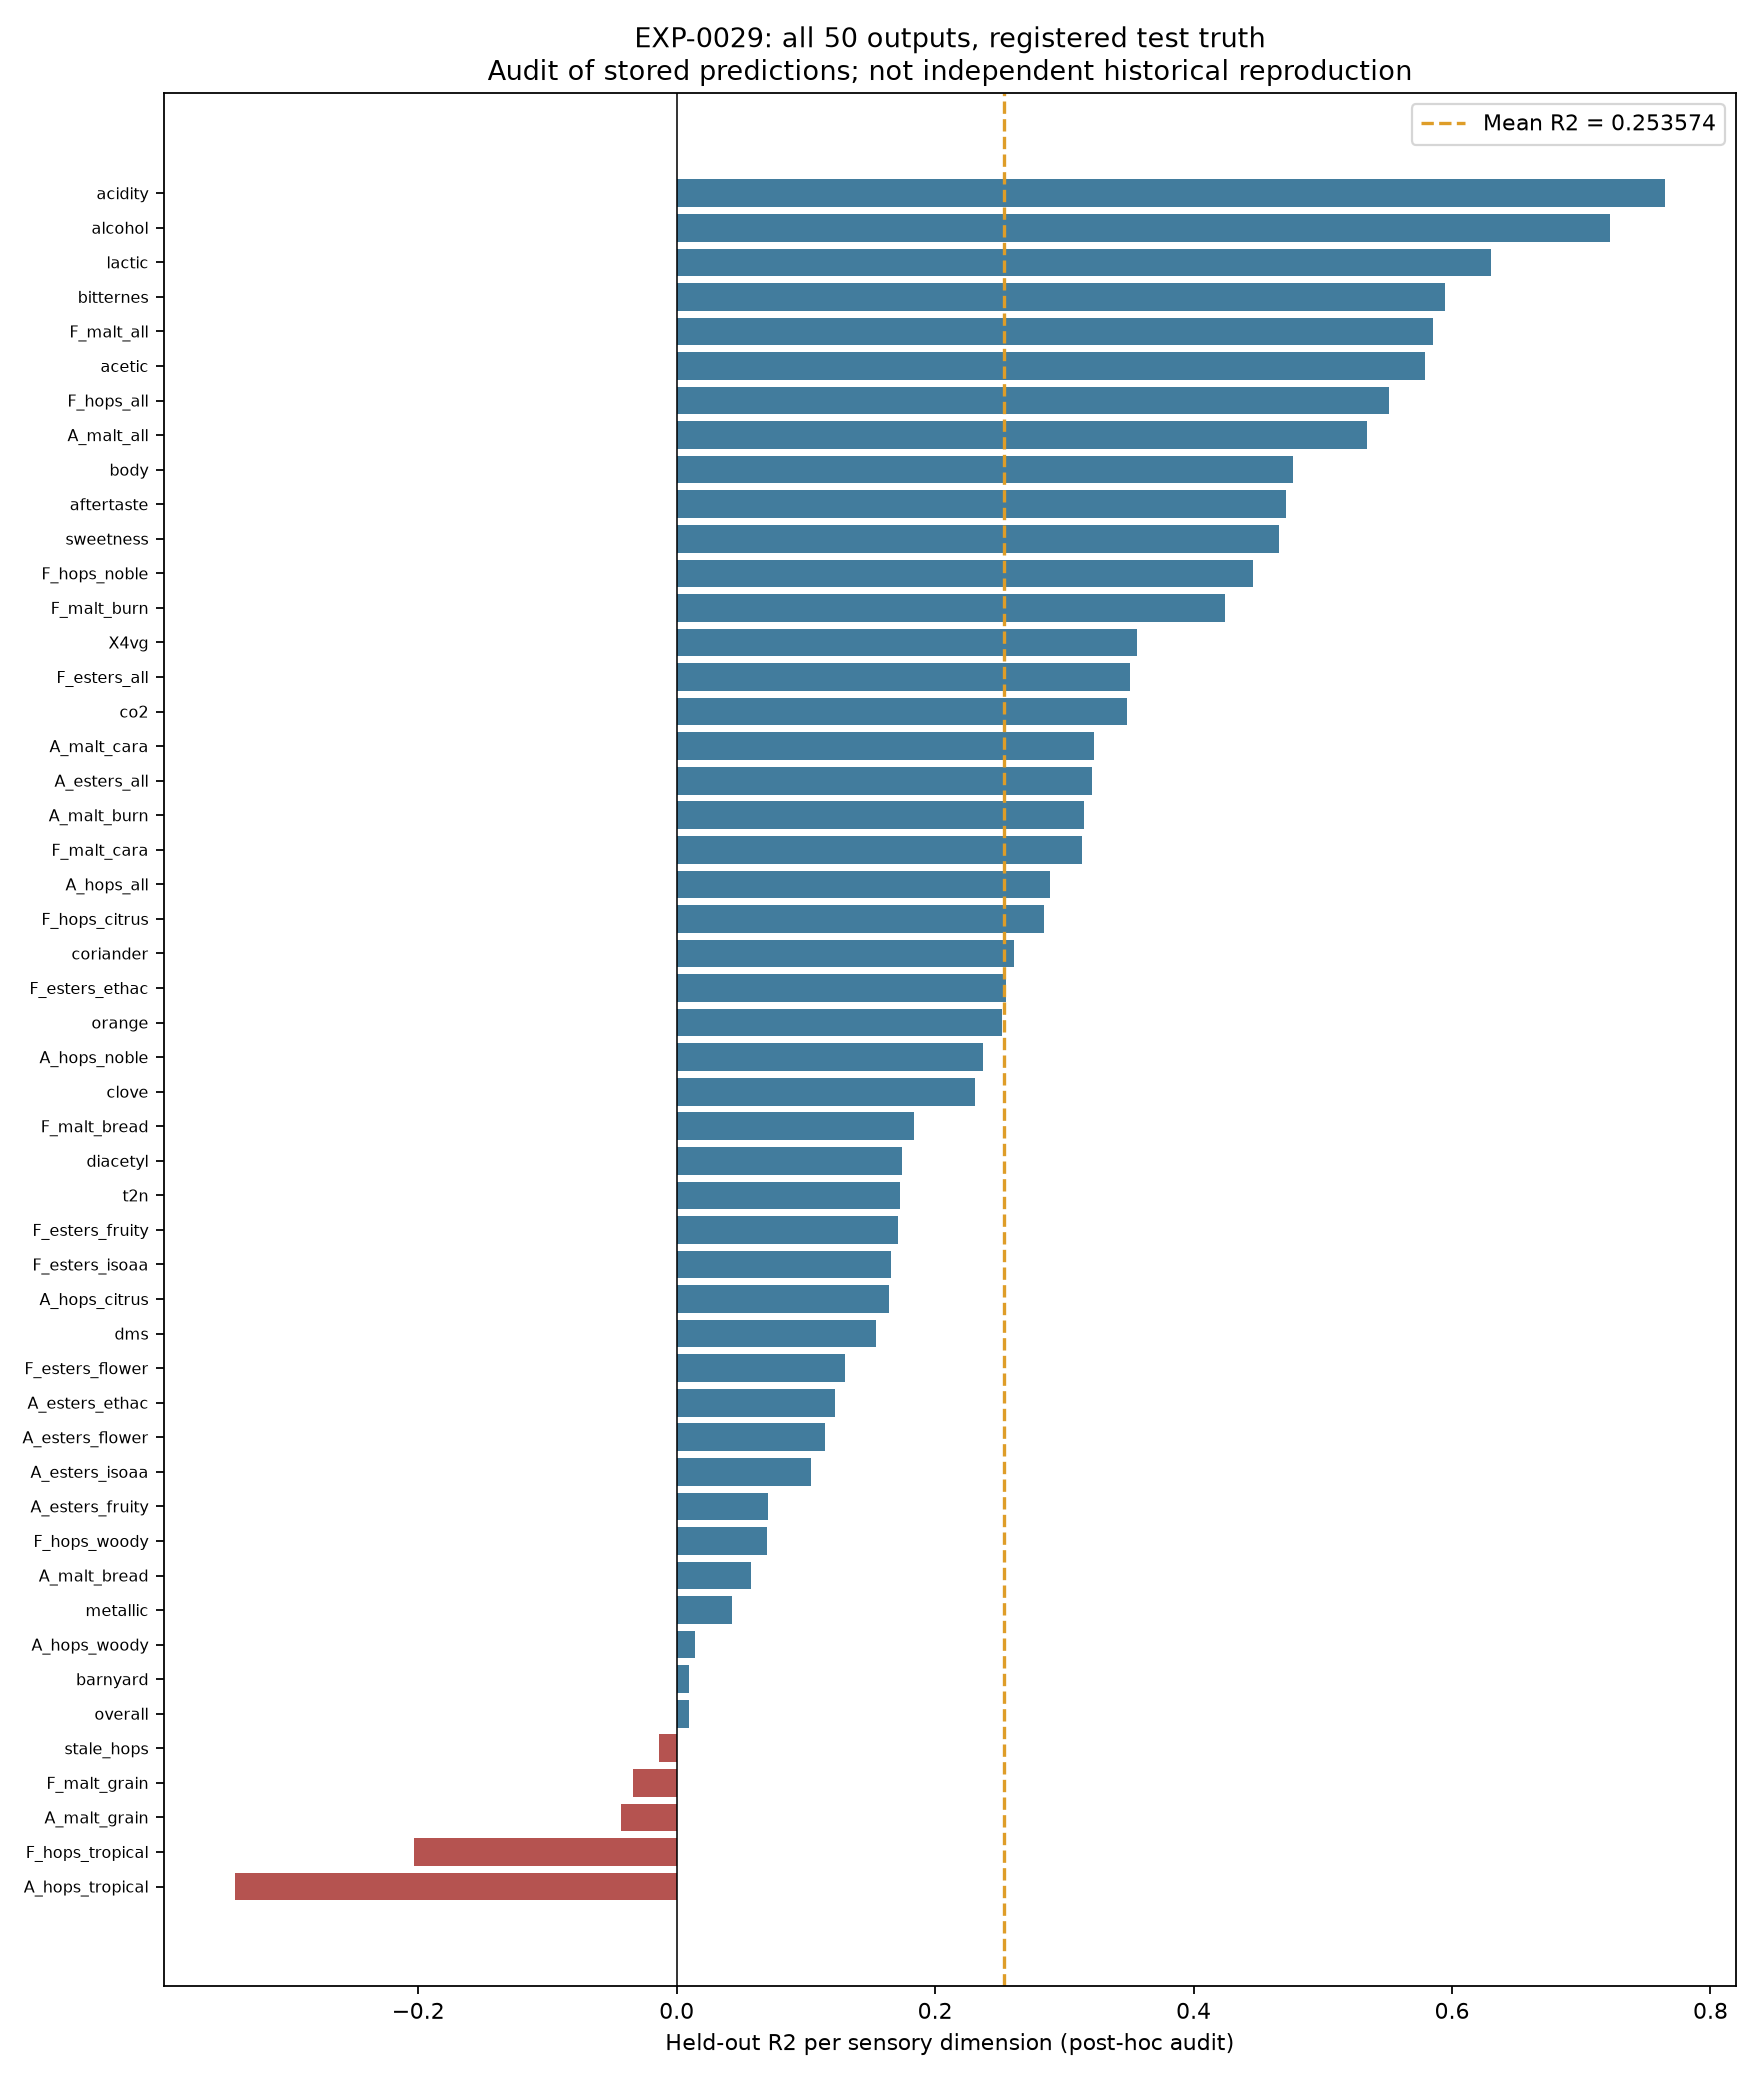
\includegraphics[width=0.72\linewidth,height=\textheight,keepaspectratio,alt={全部50维R²的事后审计}]{../figures/practical-q1-audit.png}
\caption{全部50维R²的事后审计}
\end{figure}

\subsubsection{新的隔离训练证据}\label{ux65b0ux7684ux9694ux79bbux8badux7ec3ux8bc1ux636e}

本轮模型自主编写 \texttt{src/q1\_trainonly.py}，在仅含 200 条训练记录的
OS 隔离环境中完成五折 OOF。\texttt{EXP-0049}
的初次执行因常数基线处理空特征时出现 TypeError
而失败，失败日志保留；模型修复脚本后执行 \texttt{EXP-0050/0051}。

{\def\LTcaptype{none} % do not increment counter
\begin{longtable}[]{@{}llrrl@{}}
\toprule\noalign{}
新实验 & 方法 & 50维平均OOF R² & 逐维平均MAE & 范围 \\
\midrule\noalign{}
\endhead
\bottomrule\noalign{}
\endlastfoot
EXP-0050 & 折内均值基线 & -0.008650 & 0.419159 & 训练集OOF \\
EXP-0051 & 折内 Ridge & 0.176100 & 0.363366 & 训练集OOF \\
\end{longtable}
}

这些实验是真实执行结果，但缺少完整目标绑定与后续审查，不能据此宣称质量闭环通过。训练
OOF
与旧留出成绩的样本范围、选择过程不同，不进行跨口径排名。已有留出集污染不因这些新实验而消失。

\subsection{Q2：关联分析与集合稳定性}\label{q2ux5173ux8054ux5206ux6790ux4e0eux96c6ux5408ux7a33ux5b9aux6027}

实际候选 \texttt{EXP-0041} 的平均 Jaccard 为 0.186667，中位数
0.150000；稳定席位为 14/144，命中率
0.097222。这支持``当前方法之间的关键变量集合一致性有限''，不支持强稳定性或因果解释。

新插件分别定义 Top-k Jaccard、重采样入选频率和完整排序
Spearman。集合重合、入选频率与排序相关性是不同统计量。正式稳健性执行尚未完成，不能把已有未执行的预登记计划写成已完成；也不能把同源矩阵的一致当成独立复核。

\subsection{Q3：约束满足、分布拟合与画像必须分开}\label{q3ux7ea6ux675fux6ee1ux8db3ux5206ux5e03ux62dfux5408ux4e0eux753bux50cfux5fc5ux987bux5206ux5f00}

当前选中 \texttt{EXP-0036} 的规则风格命中率为
0.994000，但这可能饱和，不能证明生成分布接近真实分布。Tripel
的能量距离比值为 0.12642884，未优于历史基线约 0.12618。迁移命中为
0.545455，对应约 6/11 个样本。

\texttt{defect\_violation\_rate} 为 0
只说明该实验定义的直接缺陷约束通过，不覆盖画像映射后的其他越阈指标。\texttt{r2\_50dim}
在旧 Q3 文件中实际上被用于画像相关性，本稿不称其为
R²。新原生检查将分布距离、数值约束满足率和训练参考群体画像 Spearman
分开计算；画像仍是代理模型一致性，不是真人喜好准确率。

历史 \texttt{VAL-0012}
等失败与上游映射器变化证据保留。没有完整冻结的历史源代码、辅助模块、模型
bundle
与标定依赖，无法补写过去的独立复跑成功。对未来新实验要求完整冻结、逐实验目录、固定种子复现，以及另行预登记的多种子稳健性。

\subsection{验证、未通过原因与最终状态}\label{ux9a8cux8bc1ux672aux901aux8fc7ux539fux56e0ux4e0eux6700ux7ec8ux72b6ux6001}

本轮质量计划实际执行后：通过 15 项、失败 10 项、待语义复核 4 项、不适用
3 项、过期 1 项。存在 18
条阻塞记录，其中包含重复或额外计划项，不能误读为同样多的独立根因。

主要根因是：历史留出集复用超限；旧实验没有完整不可变依赖；Q1
分数变换尚未独立审查；已声明目标与旧 baseline
记录未绑定；三个稳健性计划没有有效执行；部分旧审查因实际对象变更而过期。Q2
已有候选，``Q2 无候选''不再是当前根因。

工程上可运行、质量检查通过、七检查点通过是三个分别成立的条件。终稿条件始终为
\texttt{engineeringComplete\ AND\ qualityPassed\ AND\ checkpointsPassed}，不是``已有
PDF''或``实验成功''。本项目保持 \texttt{final=false}，只能生成显式 DRAFT
包。

\subsection{模型自主、工程辅助与费用边界}\label{ux6a21ux578bux81eaux4e3bux5de5ux7a0bux8f85ux52a9ux4e0eux8d39ux7528ux8fb9ux754c}

模型自主：修订三个目标契约、编写训练 OOF
脚本、修复一次真实失败、执行均值与 Ridge 实验、编写完整 50
维事后审计脚本。工程辅助：一致快照、预算接缝、执行审计
wrapper、生成本审计草稿与图、编译格式、运行质量检查和草稿打包。

模型在准备一次工具调用时输出了非 JSON 的占位变量，宿主返回
MALFORMED\_RESPONSE。该次尝试未提供原生用量，因此已停止所有新付费验收；独立模型审查、模型自主
claim/coverage/robustness/review 全闭环尚未完成。已确认累计 3,389,231
tokens，另有 1,056,768 tokens 请求预留未能结算，实际总量未知，保守上界为
4,445,999 tokens。未使用剩余预算继续重试。

\subsection{复现与证据}\label{ux590dux73b0ux4e0eux8bc1ux636e}

原项目为只读来源；所有本轮整理发生在独立副本。先核验
\texttt{SOURCE-SNAPSHOT.json} 与输出审计 SHA，再在固定 Python
环境中运行审计
wrapper。训练实验从各自冻结源目录执行，必须使用登记种子和训练输入，不得读取原测试文件。不要直接运行旧生成脚本覆盖共享输出。

Q1 审计文件、公开 handler
回执、真实宿主模型工具回执、阶段费用账和完整质量报告随交付附上。本稿不是新的模型自主终稿，也没有通过改动台账、放松质量门或提高留出次数来制造成功。

\end{document}
